\begin{coverpage}{Zulip - a Communication Platform for Collaborations}
{
\subsubsection*{What is Zulip?}
\textbf{Zulip} stands out as a dynamic and free communication platform, offering a structured and organized way of messaging, similar to Slack.

\begin{figure}[h]
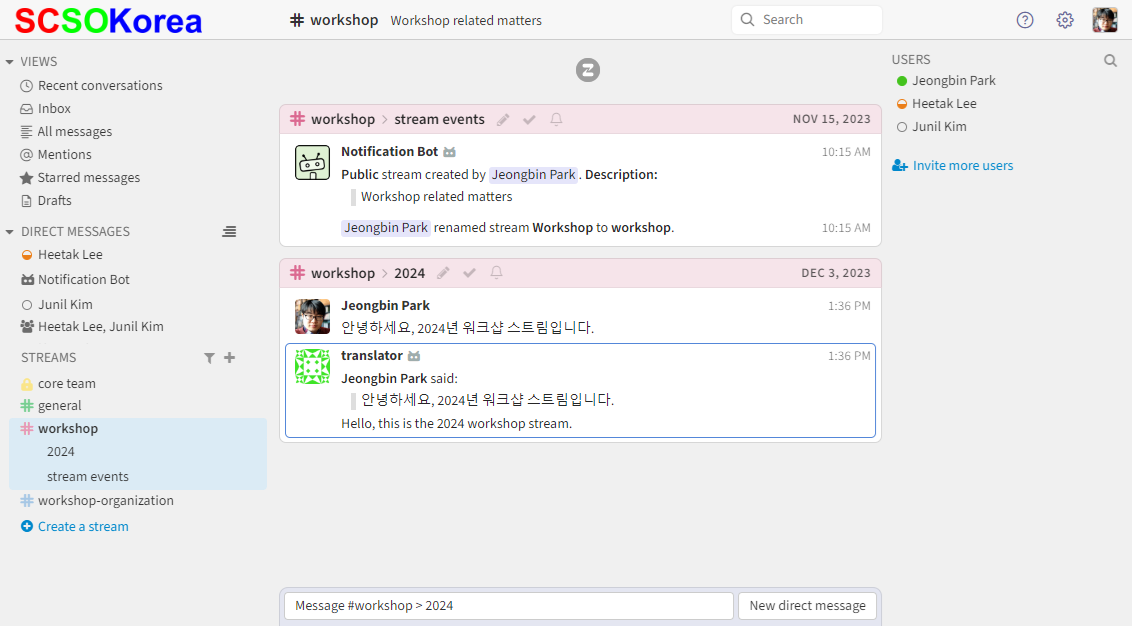
\includegraphics[width=\textwidth]{images/zulip.png}
\end{figure}

Currently, our Zulip instance is self-hosted by the Computational Omics Laboratory at Pusan National University. This means it is completely \textbf{free}, and has no bulls**t, e.g., a 90-day message limit.

Moreover, it comes with a Korean-to-English translator (based on Papago translator - thanks to Dr. Heetak Lee for providing an account for this), which automatically translates your Korean messages into English, so that you can even use Korean to communicate with English-speaking collaborators.
\\
\begin{table}[h]
\begin{tblr}{
  colspec = {Xccc},
  row{1} = {font=\bfseries},
  hlines,
}
\textbf{Feature} & \textbf{Zulip} & \textbf{Slack} & \textbf{KakaoTalk} \\
Friendly User Interface & O & O & O \\
Real-time Communication & O & O & O \\
File Sharing & O & O & O \\
Multi-platform & O & O & {X \\ \footnotesize(no Linux support)} \\
Integrations & O & O & X \\
Bots (e.g., translators) & O & O & X \\
Customizability & O & O & X \\
Unlimited Message History & O & X & X \\
Open Source & O & X & X \\
\end{tblr}
\end{table}

Thus we strongly recommend you to use Zulip as a robust and free alternative to other means of communication between institutions for your research. We hope that Zulip becomes your favorite go-to platform for effective, efficient collaboration within our community and beyond.

\subsection*{1. How to Register and Log In}
First, you need to install a mobile or desktop app. Zulip is accessible on various platforms, including Windows, macOS, Linux, Android, and iOS.
\newpage

\begin{figure}[h]
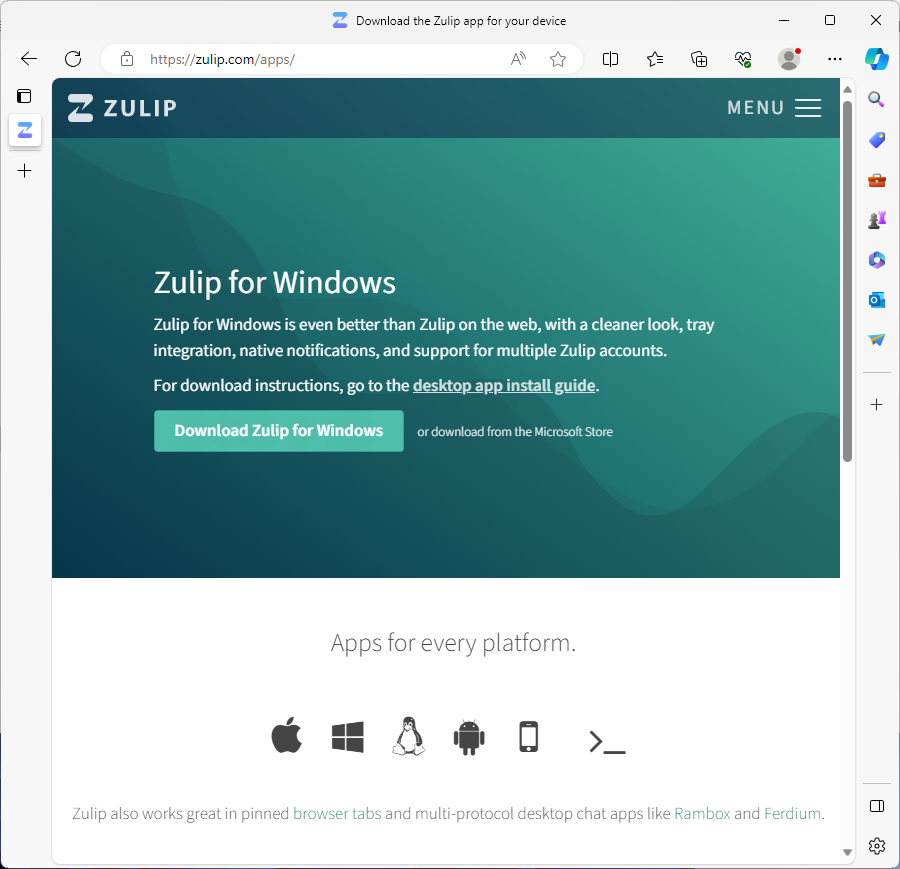
\includegraphics[width=\textwidth]{images/zulip-apps.png}
\end{figure}

{\centering \noindent Visit \textbf{\texttt{https://zulip.com/apps/}} to install the suitable one.}
\\
\\
After that, open the installed app and follow the below instructions:
\begin{itemize}[leftmargin=0.5cm, rightmargin=0.5cm]
\item \textbf{Enter the Zulip Server URL:} Open Zulip app, and type \\ \textbf{\texttt{https://zulip.scsok.io/}}. Click \textbf{\texttt{Connect}}.
\begin{figure}[h]
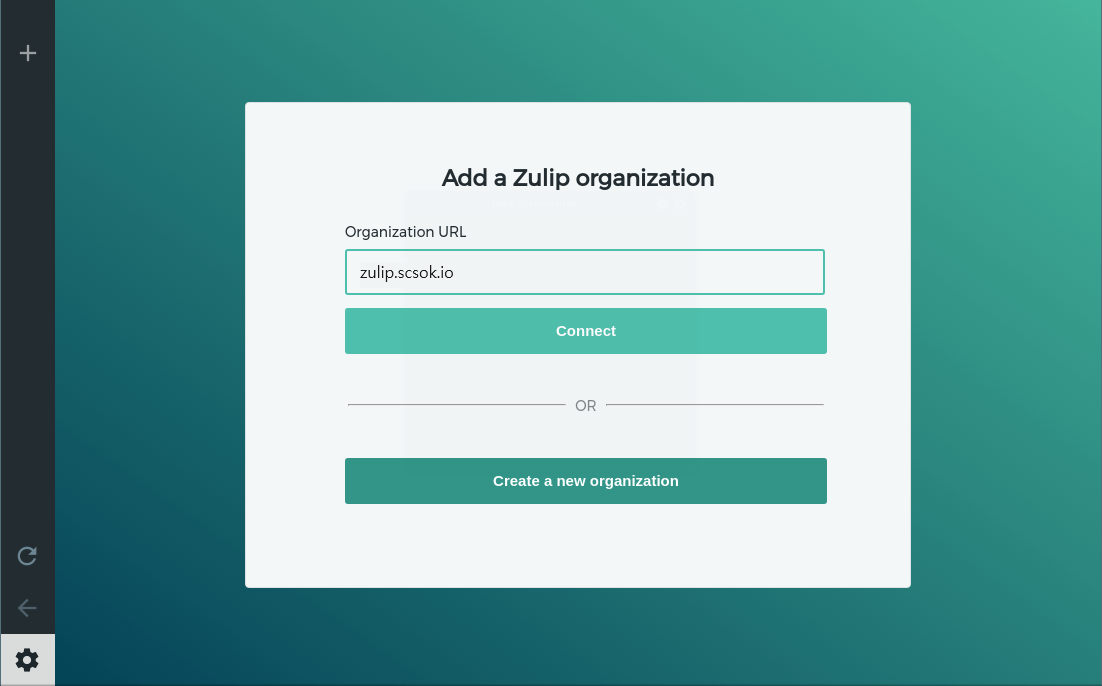
\includegraphics[width=\textwidth]{images/zulip-new-url.png}
\end{figure}
\item \textbf{Sign Up:} Click \textbf{\texttt{Sign Up}} and use your email or GitHub account to register.
\item \textbf{Log In:} Enter your credentials to sign in.
\end{itemize}
\subsection*{2. Sending Messages in Streams}
Zulip organizes messages into \textbf{Streams}. As a new user, you'll automatically join the \textbf{general}and \textbf{workshop} streams. The \textbf{workshop} stream is particularly important for our purposes; it's where we'll post announcements, hold discussions, and have Q\&A sessions.

\begin{figure}[h]
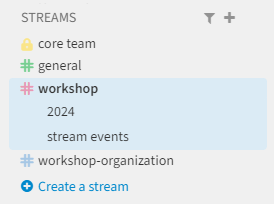
\includegraphics[width=7.5cm]{images/zulip-streams.png}
\centering
\end{figure}

Each stream is further divided into \textbf{Topics}. These act like subcategories, helping to keep conversations organized. For instance, within the \textbf{workshop} stream, there's a topic named \textbf{2024}. All messages related to the workshop in 2024 will be found here.

By default, Zulip doesn't send push notifications for every new message in a stream. If you prefer to stay more closely updated, especially for certain topics, you can adjust your notification settings. Simply set the notification preference for a topic to \textbf{Follow} and you'll be notified of new messages on that topic.

\begin{figure}[h]
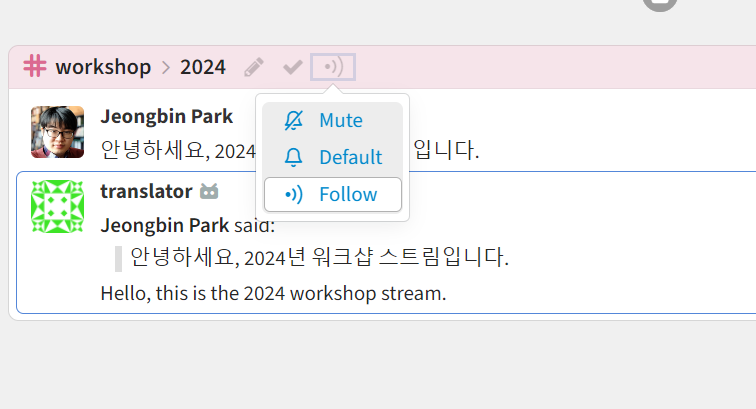
\includegraphics[width=\textwidth]{images/zulip-follow.png}
\centering
\end{figure}

\begin{itemize}[leftmargin=0.5cm, rightmargin=0.5cm]
\item \textbf{Join a Stream:} Find and join relevant streams.
\item \textbf{Send Messages:} Use the input box to type messages.
\item \textbf{Change Notifications Settings:} Customize notification settings on topics you are interested in.
\end{itemize}
\subsection*{3. Sending Direct Messages to Each Other}
Apart from the stream-based communication in Zulip, there's also the option to send \textbf{Direct Messages} to individual users or small groups. This feature works similarly to other instant messaging services like KakaoTalk. When you use Direct Messages, your conversation is private and can only be seen by the people involved in the chat.

\begin{figure}[h]
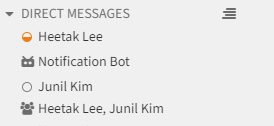
\includegraphics[width=7.5cm]{images/zulip-dm.png}
\centering
\end{figure}

Another key aspect of Direct Messages in Zulip is that you will receive push notifications for all of them. This ensures that you won't miss any personal or direct communications, as you'll be alerted each time you receive a new message on your mobile device. This is different from the default setting for streams, where you need to opt in for notifications.
\begin{itemize}[leftmargin=0.5cm, rightmargin=0.5cm]
\item \textbf{Find a User:} Click 'New Private Message'.
\item \textbf{Enter Recipient:} Add the recipients' name.
\item \textbf{Compose and Send:} Write and send your message.
\end{itemize}
\subsection*{4. How to Create a New Stream for Your Collaboration}
In Zulip, you also have the flexibility to create new streams for collaborations between different institutions. When setting up a new stream, you can choose to make it private. This means that the stream will be visible only to those who are invited or added by the stream's creator or administrators. This feature is particularly useful for projects or conversations that require confidentiality or are limited to a specific group of participants.

In addition, you can invite a "translator" bot to your streams. This bot automatically translates messages containing Hangul, facilitating communication in multilingual settings.
\begin{itemize}[leftmargin=0.5cm, rightmargin=0.5cm]
\item \textbf{Create Stream:} Access 'Streams' > 'Create Stream'.
\item \textbf{Set Details:} Name your stream and add a description.
\item \textbf{Add Members:} Invite collaborators.
\item \textbf{Configure:} Adjust privacy and settings.
\end{itemize}
}
\end{coverpage}
